\documentclass[conference]{IEEEtran}
\usepackage{cite}
\usepackage{amsmath,amssymb,amsfonts}
\usepackage{graphicx}
\usepackage{textcomp}
\usepackage{xcolor}
\usepackage{booktabs}
\usepackage{multirow}
\usepackage[T1]{fontenc}
\usepackage{url}
\graphicspath{{../figures/en/}}
\def\BibTeX{{\rm B\kern-.05em{\sc i\kern-.025em b}\kern-.08em
    T\kern-.1667em\lower.7ex\hbox{E}\kern-.125emX}}
\begin{document}

\title{Co-Optimizing Virtual Power Lines and Virtual Data Centers in Day-Ahead Unit Commitment for Thermal-Dominated Systems with High Renewable Penetration}

\author{\IEEEauthorblockN{1\textsuperscript{st} Guilherme Steilein}
\IEEEauthorblockA{\textit{Dept. of Electrical Eng.} \\
\textit{Univ. Federal do Paran\'a}\\
Curitiba, Brazil \\
steilein@ufpr.br}
\and
\IEEEauthorblockN{2\textsuperscript{nd} Clodomiro Unsihuay-Vila}
\IEEEauthorblockA{\textit{Dept. of Electrical Eng.} \\
\textit{Univ. Federal do Paran\'a}\\
Curitiba, Brazil \\
clodomiro.vila@ufpr.br}
\and
\IEEEauthorblockN{3\textsuperscript{rd} Flavio Arthur Ferreira}
\IEEEauthorblockA{\textit{Dept. of Electrical Eng.} \\
\textit{Univ. Federal do Paran\'a}\\
Curitiba, Brazil \\
flavio.ferreira@ufpr.br}
}

\maketitle

\begin{abstract}
Thermal-dominated systems absorbing large shares of variable renewable energy (VRE) face a compound problem: corridors saturate during renewable peaks, curtailment rises, and thermal units are cycled to follow net load. Two non-wire resources address it through opposite mechanisms: a Virtual Power Line (VPL), a pair of battery energy storage systems at the two ends of a congested corridor, moves \emph{energy} in time; a Virtual Data Center (VDC), a set of distributed data-center sites executing deadline-constrained workloads, moves \emph{load} in space and time. This paper proposes a network-constrained day-ahead unit commitment (UC) that co-optimizes both resources with thermal generation. The VDC is modeled per workload, with job energy, execution window, feasible sites and asymmetric migration costs, which separates temporally from spatially flexible jobs. Case studies on the RTS-GMLC system under 30--70\% VRE penetration quantify each resource and their interaction, including---distinctively---thermal cycling. Solved to a 0.05\% MIP gap, required for the interaction to be distinguishable from solver tolerance, the results show that two flexibilities relieving the same bottleneck compete economically although they provide different services: the VPL acts mainly on curtailment and the VDC on thermal cycling, yet the mean interaction is negative at every penetration level and grows beyond the optimization-gap uncertainty with VPL size: with a 400~MW VPL the joint benefit falls 19--28\% of the load-flexibility benefit short of the sum, and about 67\% at 650~MW at base VDC sizing; at base VPL sizing the shortfall is of the order of that uncertainty. On four representative days, joint deployment reduces operating cost by 6.2\%, curtailment by 12\% and thermal start-ups by 41\%; on twelve additional monthly days the reductions are 4.6\%, 15\% and 47\%. A decomposition shows that 96\% of the emergent VPL benefit is captured by the two terminal batteries acting independently, so the result is not specific to coordinated VPL operation.
\end{abstract}

\begin{IEEEkeywords}
Unit commitment, virtual power line, battery energy storage, data center load flexibility, spatiotemporal load shifting, renewable curtailment, transmission congestion, thermal cycling.
\end{IEEEkeywords}

\section{Introduction}

\IEEEPARstart{L}{atin} American power systems are adding wind and solar capacity far faster than the transmission that connects it to load centers. In Brazil, wind and solar concentrated in the Northeast must reach the Southeast through long corridors, and generation cut-offs (\emph{constrained-off}) imposed for network reasons have become a recurrent operating condition \cite{ons2025curt}; in Chile, solar from the Atacama flows south to the central load pocket and curtailment of variable renewables reached 5.9~TWh in 2024, 2.5 times the 2023 level \cite{cen2025reporte}. In both systems a thermal fleet built for energy security increasingly operates as the ramping reserve that follows net load. Because a new high-voltage line takes the better part of a decade to license and build, operators are turning to non-wire alternatives that can be deployed in months and act directly on congestion \cite{irena2020vpl}.

Two such alternatives are examined here: the \emph{Virtual Power Line} (VPL), also called virtual transmission line (VTL) or grid booster, a pair of battery energy storage systems (BESS) at the ends of a congested corridor operated so that the pair emulates transfer capacity \cite{irena2020vpl,aguero2024,wang2025vt,wang2025stoch,vpl2024epsr,ferreira2025,ferreira2026}; and what we term a \emph{Virtual Data Center} (VDC), a fleet of distributed data-center sites whose deferrable workloads can run at a different time or site \cite{liu2015glb,lindberg2022,zhang2021remunerating,wan2026scuc,riepin2024}. Data centers are among the fastest-growing loads in the region, and whether to connect them as firm load or as flexible resources is an open regulatory question.

Each resource has been studied in isolation. Deterministic and stochastic SCUC models show that a BESS pair can outperform both a new line and a standalone BESS in cost and congestion relief \cite{wang2025vt,wang2025stoch}; MILP dispatch models couple charge/discharge modes to line-flow status \cite{vpl2024epsr}; field assessments quantify the transfer-capacity boost \cite{aguero2024}. The authors' previous work embedded VPLs and inter-area VTLs in robust expansion planning with a soft-linked UC layer, showing on the RTS-GMLC system that an inter-area VTL defers trunk-line reinforcement by several years \cite{ferreira2025,ferreira2026}; the present paper translates that planning-level concept into an operational tool. On the data-center side, spatiotemporal flexibility has been embedded in SCUC through an aggregate flexibility ratio \cite{wan2026scuc} and capacity-expansion studies show that temporal flexibility reduces cost but not necessarily emissions \cite{senga2026}, on a base of geographical load balancing \cite{liu2015glb}, its carbon impact \cite{lindberg2022}, market remuneration \cite{zhang2021remunerating} and 24/7 carbon-free matching \cite{riepin2024}.

Three gaps remain. First, to the authors' knowledge VPL and VDC have not been co-optimized in the same scheduling model, so it is not known whether they are complements or substitutes---both arbitrate the same congested corridor, one from the supply and one from the demand side. Second, data-center flexibility in UC has been represented as an aggregate energy budget \cite{wan2026scuc}, which cannot capture per-workload deadlines, site eligibility or asymmetric migration costs. Third, the operational studies cited above do not report thermal cycling or ramping headroom, the quantities flexibility is supposed to relieve in thermal-dominated systems; ramp-surplus metrics appear at planning level \cite{ferreira2026}.

The contributions of this paper are: (i)~a network-constrained day-ahead UC that co-optimizes a VPL and a VDC with thermal generation, with an interaction metric---joint benefit minus the sum of individual benefits---and the solver precision required to measure it; (ii)~an energy-based per-workload VDC model with hard execution window, feasible-site set, PUE and asymmetric migration cost, in which jobs are divisible and preemptible, and which separates temporal and spatial flexibility by construction; (iii)~an assessment on the RTS-GMLC system, on the stressed inter-area corridor of \cite{ferreira2026}, across 30--70\% VRE penetration and a two-dimensional sizing sweep; and (iv)~an implementation in PyPSA \cite{brown2018pypsa} that reproduces all results.

\section{Two Congestion Arbitrageurs}
\label{sec:concepts}

Consider a corridor $\ell$ from a renewable-rich exporting area to an importing load area, with thermal limit $F_\ell$. When it saturates, renewable output is curtailed upstream or thermal units are committed downstream to serve load that could otherwise be imported. A \textbf{VPL} places a BESS at each terminal: the upstream unit absorbs energy that could not be transferred and the downstream unit discharges when the corridor is saturated, shifting energy across the corridor in time---a time-varying increase in transfer capability \cite{irena2020vpl,wang2025vt}. In \cite{ferreira2026} the mode of each terminal BESS is fixed by a switching rule on flow direction and net-demand stage; here the VPL is represented by default as two uncoupled storage units and the explicit rule is kept as an option.

A \textbf{VDC} is a set $\mathcal{D}$ of data-center sites operated as one flexible resource. Site $d$ has electrical capacity $C_d$, power usage effectiveness $\mathrm{PUE}_d$ and a non-deferrable base load; the deferrable part is a set $\mathcal{J}$ of workloads, job $j$ requiring energy $E_j$ (IT load) within a window $[a_j,b_j]$ at any site of a feasible set $\mathcal{D}_j$, at a migration cost $c_{j,d}$ per electrical MWh, asymmetric as inter-site bandwidth and latency are. \emph{Batch} jobs (long window, native site) provide temporal flexibility, \emph{migratable} jobs (short window, any site) spatial flexibility. Unlike an aggregate flexible fraction of daily energy \cite{wan2026scuc}, deadlines are hard constraints.

Both resources respond to the locational value created by congestion and compete for the same corridor opportunity: the VPL and the migratable part of the VDC need corridor capacity in the same saturated hours, while batch workloads also exploit intertemporal net-load variation. If the first resource uses up that opportunity the second adds little (substitutes); if the VPL is energy-limited and the VDC window-limited, each serves a different part of it (complements). Which regime prevails is the empirical question of Section~\ref{sec:results}.

\section{Problem Formulation}
\label{sec:model}

\subsection{Nomenclature}
Sets: $\mathcal{T}$ hourly periods; $\mathcal{G}$ thermal units, $\mathcal{R}$ renewable units, $\mathcal{L}$ lines, $\mathcal{B}$ storage units, $\mathcal{D}$ data-center sites, $\mathcal{J}$ workloads; a subscript $n$ restricts a set to bus $n$. Continuous variables: $p_{g,t}$ thermal output; $r_{i,t}$ renewable output; $f_{\ell,t}$ line flow; $\theta_{n,t}$ bus angle; $p^{\mathrm{ch}}_{b,t}, p^{\mathrm{dis}}_{b,t}, e_{b,t}$ storage charge, discharge and energy; $x_{j,d,t}$ IT power of workload $j$ at site $d$; $q_{g,t}$ spinning reserve. Binaries: $u_{g,t}$ status, $v_{g,t}$ start-up, $w_{g,t}$ shut-down. Parameters: $C^{\mathrm{E}}_g, C^{\mathrm{SU}}_g, C^{\mathrm{SD}}_g$ energy, start-up and shut-down costs; $\underline{P}_g,\overline{P}_g$ output limits; $RU_g, RD_g$ ramp limits; $UT_g, DT_g$ minimum up/down times; $\bar{r}_{i,t}$ available renewable output; $F_\ell, x_\ell$ line limit and reactance; $L_{n,t}$ inflexible load; $\eta_b, \overline{P}_b, \overline{E}_b, e_{b,0}$ storage efficiency, limits and initial energy (a free variable, since the cycle is closed); $C^{\mathrm{deg}}_b$ degradation cost; $C^{\mathrm{curt}}$ curtailment penalty; $E_j, a_j, b_j, \mathcal{D}_j, c_{j,d}$ workload data; $C_d, \mathrm{PUE}_d, L^{\mathrm{DC}}_{d,t}, \Delta_d, \Delta^{\mathrm{w}}_d$ site capacity, PUE, inflexible data-center load, and IT ramp limits per site and per workload; $f_d$ flexible fraction of $C_d$; $R_t, \alpha, \gamma, \phi$ reserve requirement, its load and renewable coefficients and the flexible-reserve flag; $\sigma_t, z_t$ grid-usage stage and flow-direction indicator of the explicit VPL rule; $\epsilon$ minimum-load tolerance.

\subsection{Objective and Thermal Units}
\begin{multline}
\min \sum_{t\in\mathcal{T}} \Big[ \sum_{g\in\mathcal{G}} \big(C^{\mathrm{E}}_g p_{g,t} + C^{\mathrm{SU}}_g v_{g,t} + C^{\mathrm{SD}}_g w_{g,t}\big) \\
+ C^{\mathrm{curt}} \sum_{i\in\mathcal{R}} (\bar{r}_{i,t} - r_{i,t})
+ \sum_{b\in\mathcal{B}} C^{\mathrm{deg}}_b p^{\mathrm{dis}}_{b,t} \\
+ \sum_{j\in\mathcal{J}}\sum_{d\in\mathcal{D}_j} c_{j,d}\, \mathrm{PUE}_d\, x_{j,d,t} \Big]
\label{eq:obj}
\end{multline}
The thermal units follow the tight MILP UC formulation of \cite{morales2013tight} as implemented in PyPSA: commitment logic $u_{g,t} - u_{g,t-1} = v_{g,t} - w_{g,t}$, minimum up and down times over $UT_g$ and $DT_g$, output limits net of the reserve contribution, $\underline{P}_g u_{g,t} \le p_{g,t} \le \overline{P}_g u_{g,t} - q_{g,t}$, and ramp limits $RU_g$, $RD_g$ relaxed by $\underline{P}_g$ in the start-up and shut-down hours. Units with a minimum up time of 8~h or more start the day online and the rest offline, the RTS-GMLC deck carrying no commitment history; Section~\ref{sec:results} reports a test with the states inherited from the previous day.

\subsection{Network and Reserve}
A linearized (DC) power flow is used, $f_{\ell,t} = (\theta_{n_1(\ell),t} - \theta_{n_2(\ell),t})/x_\ell$, $|f_{\ell,t}| \le F_\ell$, with nodal balance for every bus $n$ and period $t$:
\begin{multline}
\sum_{g\in\mathcal{G}_n} p_{g,t} + \sum_{i\in\mathcal{R}_n} r_{i,t} + \sum_{b\in\mathcal{B}_n} \big(p^{\mathrm{dis}}_{b,t} - p^{\mathrm{ch}}_{b,t}\big) - \sum_{\ell} A_{n\ell} f_{\ell,t} \\
= L_{n,t} + \sum_{d\in\mathcal{D}_n}\Big( L^{\mathrm{DC}}_{d,t} + \mathrm{PUE}_d \sum_{j:\, d\in\mathcal{D}_j} x_{j,d,t} \Big),
\label{eq:balance}
\end{multline}
where $A$ is the bus--branch incidence matrix and $0 \le r_{i,t} \le \bar{r}_{i,t}$. Spinning reserve is
\begin{align}
\sum_{g\in\mathcal{G}} q_{g,t} + \phi \Big[ \sum_{b\in\mathcal{B}}\big(\overline{P}_b - p^{\mathrm{dis}}_{b,t}\big) + \sum_{j,d} \mathrm{PUE}_d\, x_{j,d,t} \Big] \ge R_t,
\label{eq:reserve}
\end{align}
with $R_t = \alpha L_t + \gamma \sum_i \bar{r}_{i,t}$, where $L_t$ is the total fixed load, i.e., $\sum_n L_{n,t}$ plus the inflexible data-center load (the deferrable part, being curtailable, does not add to the requirement); the flag $\phi\in\{0,1\}$ enables the contribution of storage headroom and curtailable data-center load to reserve ($\phi=0$ in the base case). That contribution is a headroom proxy, not a deliverability model: it checks neither the post-event deadline feasibility of a curtailed job nor the state of charge behind a storage pledge.

\subsection{Virtual Power Line}
For each storage unit $b$ of the VPL pair, with $\eta_b = \sqrt{0.85}$ so that the round-trip efficiency is 85\%,
\begin{align}
e_{b,t} &= e_{b,t-1} + \eta_b\, p^{\mathrm{ch}}_{b,t} - p^{\mathrm{dis}}_{b,t}/\eta_b, \label{eq:soc}\\
0 \le e_{b,t} &\le \overline{E}_b, \quad 0 \le p^{\mathrm{ch}}_{b,t},\, p^{\mathrm{dis}}_{b,t} \le \overline{P}_b, \quad e_{b,|\mathcal{T}|} = e_{b,0}.
\end{align}
In the emergent formulation no constraint couples the two units or forbids simultaneous charging and discharging; with $C^{\mathrm{deg}}_b = 2$~\$/MWh and $C^{\mathrm{curt}} = 0.1$~\$/MWh, dissipating energy in the battery is never profitable, and an ex-post check of every solution confirms $\min\{p^{\mathrm{ch}}_{b,t}, p^{\mathrm{dis}}_{b,t}\} = 0$ for all VPL units and hours. In the explicit variant, following \cite{ferreira2026}, a binary indicator $z_t$ of flow direction and a stage parameter $\sigma_t\in\{0,1\}$ (net demand above the 90th or below the 30th percentile of the daily duration curve) fix the mode of each terminal unit,
\begin{align}
p^{\mathrm{ch}}_{b^{\downarrow},t} \le \overline{P}_b\,(1 - z_{t}), \quad p^{\mathrm{dis}}_{b^{\uparrow},t} \le \overline{P}_b\,(1 - z_{t}), \label{eq:vtl_explicit}
\end{align}
with $z_t = 1$ when the flow is downstream: when $\sigma_t=1$ the downstream unit may only discharge and the upstream unit may only charge; when $\sigma_t=0$ the roles are reversed ($p^{\mathrm{dis}}_{b^{\downarrow},t} \le \overline{P}_b z_t$, $p^{\mathrm{ch}}_{b^{\uparrow},t} \le \overline{P}_b z_t$); intermediate hours are free for arbitrage. The rule is linearized with big-$M$ as in \cite{ferreira2026}.

\subsection{Virtual Data Center}
For each workload $j$, site $d\in\mathcal{D}_j$ and period $t$:
\begin{align}
\sum_{d\in\mathcal{D}_j} \sum_{t=a_j}^{b_j} x_{j,d,t} &= E_j, \qquad x_{j,d,t} = 0 \;\; \forall t \notin [a_j, b_j], \label{eq:energy}\\
\sum_{j:\, d\in\mathcal{D}_j} \mathrm{PUE}_d\, x_{j,d,t} &\le C_d - L^{\mathrm{DC}}_{d,t} \quad \forall d,t, \label{eq:site}\\
\Big| \sum_{j} x_{j,d,t} - \sum_{j} x_{j,d,t-1} \Big| &\le \Delta_d \quad \forall d,t, \label{eq:ramp}\\
\big| x_{j,d,t} - x_{j,d,t-1} \big| &\le \Delta^{\mathrm{w}}_d \quad \forall j, d\in\mathcal{D}_j, t. \label{eq:rampjob}
\end{align}
Equation \eqref{eq:energy} is the hard deadline, \eqref{eq:site} the site capacity net of inflexible load, \eqref{eq:ramp} the hourly ramp of the aggregate IT load at a site and \eqref{eq:rampjob} the ramp of a single workload at it. They are separate parameters because provisioning is rate-limited per migration stream as well as in aggregate: a workload cannot enter or leave a site instantaneously even at constant site total. We set $\Delta^{\mathrm{w}}_d = \Delta_d$. Because $x_{j,d,t}$ is continuous, jobs are divisible across hours and sites and preemptible at no cost, an upper bound on the flexibility of non-preemptible jobs, which would require activation binaries. In PyPSA each workload is a virtual bus fed by one link per eligible site (efficiency $1/\mathrm{PUE}_d$, availability window, migration cost) and terminated by a store whose minimum energy jumps to $E_j$ at the deadline; \eqref{eq:site} and \eqref{eq:ramp} are added as custom constraints and \eqref{eq:rampjob} is the link's native ramp limit. It is not redundant: it is active in all 160 VDC instances and in 8.7\% of the workload--site/hour pairs, a third away from a window edge.

\subsection{Cases and Interaction Metric}
\label{sec:metrics}
Four cases are solved for every day and penetration level: (A) base UC without either resource; (B) A + VPL; (C) A + VDC; (D) A + VPL + VDC. In A and B the data-center energy is present but inflexible: each site is a flat load carrying exactly the daily energy that the generated workloads consume in C and D, so cost differences measure the value of flexibility relative to a smooth inflexible profile; a stricter baseline, in which the same jobs run at their native site from arrival, is tested in Section~\ref{sec:results}. Let $\Delta_X$ denote the reduction of a metric in case $X$ relative to A (negative if the metric worsens). The interaction is
\begin{align}
I = \Delta_D - (\Delta_B + \Delta_C),
\label{eq:interaction}
\end{align}
with $I<0$ indicating substitution and $I>0$ complementarity. Because $I$ is a difference of four MILP objectives, it is only meaningful when it exceeds the sum of the absolute optimality gaps of the four solutions; this \emph{gap noise} is reported alongside $I$. The metrics are: operating cost; curtailment $\sum_{i,t}(\bar r_{i,t}-r_{i,t})$; start-ups $\sum_{g,t} v_{g,t}$; minimum-load unit-hours $\sum_{g,t} \mathbb{1}[p_{g,t} \le (1+\epsilon)\underline{P}_g u_{g,t}]$, $\epsilon=10^{-3}$; flexible ramp-up/down surplus (FRUS/FRDS) as defined in \cite{ferreira2026}, averaged over committed units and hours; corridor congestion hours $\sum_t \mathbb{1}[|f_{\ell,t}| \ge 0.98 F_\ell]$; mean LMP spread across the corridor terminals, from a linear re-solve with the commitment fixed; virtual capacity $\sum_t p^{\mathrm{dis}}_{b^{\downarrow},t}\mathbb{1}[|f_{\ell,t}| \ge 0.98F_\ell]$ of the downstream unit; energy shifted spatially (outside the native site) and temporally (outside the arrival hour); and CO$_2$ from fuel-specific factors.

\section{Case Study}
\label{sec:case}

\textbf{Test system.} The RTS-GMLC system \cite{barrows2020rts} is used: 73 buses in three areas, 120 branches, 158 units (nuclear, treated as must-run, coal, gas combined-cycle and combustion turbines, oil, hydro) and hourly day-ahead renewable profiles. Thermal cost curves are linearized at 80\% of rated output, with cold start-up costs. The stressed configuration of \cite{ferreira2026} is adopted for comparability with the planning study: load in Area~2 is increased by 40\% and an equivalent capacity (1140~MW, 70\% wind) is added in Area~3 at its candidate buses, which turns the inter-area trunk 318--223 (500~MW) into the binding corridor. Renewable capacities are scaled by a single annual factor so that available renewable energy equals 30, 50 or 70\% of annual load, as in \cite{ferreira2026}. On the high-wind spring day at 50\% the corridor is at its limit for 11 of 24 hours in the base case.

\textbf{Flexibility resources.} The VPL consists of two BESS at buses 318 (upstream) and 223 (downstream), 200~MW / 4~h each in the base case, 85\% round-trip efficiency as in \cite{ferreira2026}, degradation cost 2~\$/MWh; the 650~MW VTL storage selected by the planning model in \cite{ferreira2026} is the upper bound of the sizing sensitivity. The VDC consists of three sites, one per area, at the largest load buses 118, 218 and 318, each with 200~MW of electrical capacity, PUE 1.30 and flexible fraction $f_d=0.5$ in the base case. The nominal deferrable energy per site and day is $0.7 f_d C_d\cdot 24$~MWh, split equally between batch and migratable workloads: $|\mathcal{J}| = 18$ jobs (per site, 2 batch with an 8--12~h window at the native site and 4 migratable with a 2--4~h window at any site), $E_j$ from a Dirichlet split, uniform arrivals and window lengths, IT ramp limits $\Delta^{\mathrm{w}}_d = \Delta_d = 0.5 f_d C_d/\mathrm{PUE}_d$. Jobs are trimmed to their window and each site scaled to be feasible under earliest-deadline-first, reducing the deferrable energy from 3877 to 3181~MWh of IT load. Migration costs are 5--20~\$ per electrical MWh, asymmetric, zero at the native site; the curtailment penalty is $C^{\mathrm{curt}} = 0.1$~\$/MWh, applied as a credit on dispatched renewable energy, which shifts every daily cost by a constant and leaves $\Delta$ and $I$ unchanged. Workloads are generated from a fixed seed and are identical across cases. The reserve requirement is $R_t = 0.03\,L_t + 0.05 \sum_i \bar r_{i,t}$.

\textbf{Study days and implementation.} Four days are selected from the annual net-demand series as in \cite{ferreira2026}: largest renewable surplus (12~March), peak load (26~August), steepest 3-h ramp (14~January) and median net-demand energy (16~March). Sensitivities vary one parameter at a time around the 50\% base, giving fourteen variations per day: penetration (30/70\%), VPL power (100/400/650~MW per terminal), flexible fraction (0.2/0.8), batch window width ($\times0.5/\times2$), migration cost ($\times0.5/\times2$), the reserve flag $\phi$ and the two switching-rule readings; a two-dimensional sweep of VPL power $\times$ flexible fraction, a decomposition of the VPL into its two terminal batteries, an alternative inflexible baseline, an initial state-of-charge test, the two switching-rule readings at 400~MW and twelve monthly days complete the design (328 instances). Models are built in PyPSA~1.3 \cite{brown2018pypsa}; each instance has 5256 binaries, 14\,040 variables and 45\,910 constraints and is solved with Gurobi~13.0 to a 0.05\% MIP gap on a 12-core laptop (median 10~s; five instances reached the 1800~s limit, at gaps of 0.05--0.12\%). Code and results: \url{https://github.com/Steilein/UC_VPL_VDC}.

\section{Results and Discussion}
\label{sec:results}

\subsection{Value of Each Resource}
Unless stated otherwise, all cases use the emergent VPL formulation. Table~\ref{tab:base} reports the four cases on the high-wind spring day at 50\% penetration, where the corridor mechanism is clearest. Renewable availability is 115~GWh against a load of 113~GWh, so 37\% is curtailed in the base case. The VPL alone reduces cost by 10.7\% and curtailment by 5.0\% and discharges 170~MWh downstream while the corridor is at its limit, but leaves start-ups unchanged: the energy it can move is bounded by 4~h of storage and it acts on the renewable surplus, not on the evening ramp. Installing each terminal battery alone yields 37.6~k\$ (upstream) and 35.9~k\$ (downstream) on average over the four days, against 76.6~k\$ for the pair: the pairing itself adds 4\% (1 to 9\% by day), so the emergent VPL benefit is essentially that of two corridor-terminal batteries acting independently. The VDC alone reduces cost by 3.6\% and curtailment by 2.7\%, yet cuts start-ups from 7 to 3: by concentrating batch execution in the midday renewable peak and moving 14\% of the deferrable IT energy (454 of 3181~MWh) to other sites, it flattens the net load. Combined, they reduce cost by 14.4\%, curtailment by 7.9\%, start-ups by 43\% and CO$_2$ by 11\%; averaged over the four days, cost falls 6.2\%, curtailment 12\% and start-ups 41\% (Table~\ref{tab:interaction}). The VDC value depends on the inflexible baseline: running the same jobs at their native site under earliest-deadline-first instead of a flat profile cuts the VDC benefit by one third to 15.9~k\$ and the joint benefit to 91.2~k\$, and moves the mean interaction from $-1.3$ to $-2.4$~k\$, changing its magnitude but not its sign on any day. Corridor congestion hours \emph{increase} with either resource (11 to 15--16 here), and the LMP spread is displaced rather than collapsed. Substitution therefore operates through shared corridor capacity in the same hours, not through a spread that one resource removes for the other.

\begin{table}[t]
\centering
\caption{Metrics for cases A--D, high-wind spring day, 50\% VRE}
\label{tab:base}
\footnotesize
\setlength{\tabcolsep}{3.5pt}
\resizebox{\columnwidth}{!}{%
\begin{tabular}{@{}lrrrr@{}}
\toprule
Metric & A & B (VPL) & C (VDC) & D (both) \\
\midrule
Operating cost (k\$) & 684.7 & 611.3 & 660.2 & 586.2 \\
Curtailment (GWh) & 42.7 & 40.6 & 41.6 & 39.4 \\
Thermal start-ups & 7 & 7 & 3 & 4 \\
Min-load unit-hours & 228 & 215 & 210 & 194 \\
Mean FRUS / FRDS (MW) & 58.5 / 20.3 & 58.0 / 20.4 & 63.3 / 20.4 & 62.3 / 20.8 \\
Corridor congested hours & 11 & 16 & 15 & 16 \\
Virtual capacity (MWh) & --- & 170 & --- & 170 \\
Spatial / temporal shift (MWh) & --- & --- & 454 / 1614 & 479 / 1469 \\
CO$_2$ (kt) & 21.1 & 20.1 & 19.9 & 18.9 \\
\bottomrule
\end{tabular}%
}
\end{table}

\subsection{Mechanism}
Fig.~\ref{fig:corridor} shows the corridor flow and the state of charge of the two BESS for case D; the explicit variant is plotted because it makes the $\sigma_t$ stages visible, and it produces the same qualitative pattern as the emergent case reported in Table~\ref{tab:base}, at 4\% higher cost on this day. The upstream unit charges at night and in hours 12--16, while the corridor is saturated and wind is curtailed in Area~3; the downstream unit charges through the corridor in the low-usage midday stage and discharges in the high-usage evening stage (hours 18--20). In cases C and D the deferrable load concentrates in hours 6--17 and the evening peak is almost empty at all three sites. When both are present the deferrable load does less of what the battery already does: the VDC in D shifts 145~MWh less in time than in C on this day, while the virtual transfer is unchanged at 170~MWh. Both compete for the same corridor capacity in the same hours, and the resource with the larger standalone benefit keeps its position.

\begin{figure}[t]
\centering
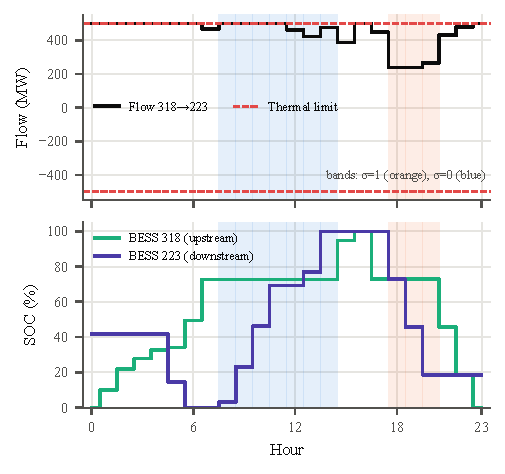
\includegraphics[width=0.72\columnwidth]{fig3_corridor_vpl.pdf}
\caption{Corridor flow vs.\ thermal limit (top) and state of charge of the two BESS (bottom), case D with the explicit rule; bands mark the high-usage ($\sigma_t=1$) and low-usage ($\sigma_t=0$) stages. End-of-hour values, so the cycle closes as $e_{b,0}=e_{b,23}$.}
\label{fig:corridor}
\end{figure}

\subsection{Interaction Across Penetration Levels}
Table~\ref{tab:interaction} reports $\Delta_B$, $\Delta_C$, $\Delta_D$ and $I$ for cost, curtailment and start-ups at 30, 50 and 70\% penetration, averaged over the four days; the gap noise of the cost interaction is 1--4~k\$ depending on the day. The mean cost interaction is negative at every level, though its magnitude is only clearly above the gap noise at 30\%: the joint benefit is 11.1\% smaller than the sum of the individual benefits at 30\%, 1.3\% at 50\% and 2.8\% at 70\%; over the 48 day--variation combinations of the main grid, $I$ is negative in 32 and exceeds twice the gap noise in 17, of which 15 indicate substitution and 2 complementarity. Substitution is strongest at 30\%, where the corridor binds in few hours (4 on average) and both resources compete for the same short window; at 50 and 70\% it binds for 9--11 hours and $I$ shrinks without changing sign. For curtailment $I$ changes sign, from $-11\%$ of the summed benefit at 30\% penetration to $+4\%$ at 50\% and $-11\%$ at 70\%; for start-ups it is negative at every level, the two resources avoiding partly the same start-ups. Because start-ups are a headline metric, the four days were re-solved with thermal states inherited from the previous day, solved as case A. Absolute counts rise (17.2 to 26.0 in case A), since fewer units are online at midnight, but so does the reduction from joint deployment (41 to 58\%), and the mean interaction becomes more negative ($-6.5$ against $-1.3$~k\$, negative on all four days): the substitution is not an artifact of the boundary condition. Twelve additional weekdays, one per month with median net-demand energy, give the same picture under less extreme conditions: cost falls 4.6\%, curtailment 15\% and start-ups 47\%, and $I$ is negative on 9 of the 12 days (mean $-2.7$~k\$). The free initial state of charge is likewise not driving the result: anchoring it at 50\% of $\overline{E}_b$ lowers the mean VPL benefit by 11\% (76.6 to 68.0~k\$) and the joint benefit to 90.6~k\$, and moves the interaction from $-1.3$ to $-1.7$~k\$/day, so the cyclic assumption is optimistic on the VPL value and conservative on the interaction. The reserve requirement is mildly asymmetric, the deferrable load counting in $L_t$ in A and B but not in C and D: imposing the A/B requirement on C and D lowers $\Delta_C$ by 0.4~k\$ and the start-up reduction from 41 to 38\%, leaving $I$ at $-1.4$~k\$/day.

\begin{table}[t]
\centering
\caption{Marginal value and interaction, mean over four days ($\Delta$ = reduction relative to case A; noise = mean gap noise of $I$, k\$)}
\label{tab:interaction}
\footnotesize
\setlength{\tabcolsep}{3.5pt}
\resizebox{\columnwidth}{!}{%
\begin{tabular}{@{}llrrrrrr@{}}
\toprule
Metric & VRE & A & $\Delta_B$ & $\Delta_C$ & $\Delta_D$ & $I$ & noise \\
\midrule
\multirow{3}{*}{Cost (k\$)} & 30\% & 1948.7 & 56.8 & 18.2 & 66.7 & $-8.3$ & 2.6 \\
 & 50\% & 1612.3 & 76.6 & 24.3 & 99.6 & $-1.3$ & 2.3 \\
 & 70\% & 1444.7 & 81.8 & 29.0 & 107.7 & $-3.1$ & 2.3 \\
\midrule
\multirow{3}{*}{Curtailment (MWh)} & 30\% & 3516 & 685 & 127 & 721 & $-91$ & --- \\
 & 50\% & 20464 & 1557 & 754 & 2407 & $+96$ & --- \\
 & 70\% & 44229 & 2057 & 891 & 2626 & $-322$ & --- \\
\midrule
\multirow{3}{*}{Start-ups} & 30\% & 17.5 & 7.2 & 5.5 & 9.2 & $-3.5$ & --- \\
 & 50\% & 17.2 & 5.5 & 7.8 & 7.0 & $-6.2$ & --- \\
 & 70\% & 18.0 & 4.5 & 4.5 & 7.0 & $-2.0$ & --- \\
\bottomrule
\end{tabular}%
}
\end{table}

\begin{figure}[t]
\centering
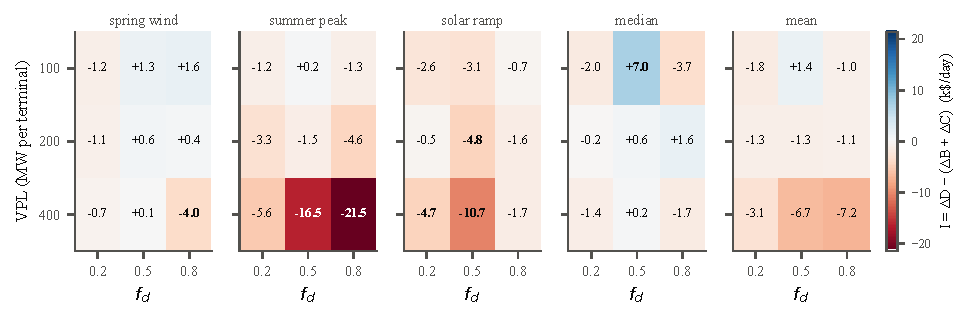
\includegraphics[width=\columnwidth]{fig8_cross_vpl_fd.pdf}
\caption{Cost interaction $I$ (k\$/day) over VPL power and flexible fraction, per day and on average; bold values exceed twice the gap noise. Negative values indicate substitution.}
\label{fig:cross}
\end{figure}

\subsection{Sensitivities and Interaction Surface}
The VPL value grows with size at a decreasing marginal rate: $\Delta_B$ rises from 38~k\$ at 100~MW to 77, 142 and 186~k\$ at 200, 400 and 650~MW (38, 32 and 18~k\$ per additional 100~MW); the planning-level 650~MW of \cite{ferreira2026} still adds value, at half the initial marginal rate. The VDC value is governed by the flexible fraction and the batch window: $\Delta_C$ is 11, 24 and 37~k\$ at $f_d = 0.2$, 0.5 and 0.8, and 8, 24 and 33~k\$ for a halved, nominal and doubled window, so the deadline is a first-order constraint. Halving or doubling the migration cost moves $\Delta_C$ by $+16$ and $-17\%$ but leaves the interaction at $-0.9$ and $-1.2$~k\$ against $-1.3$, so the result does not hinge on that parameter. Reserve provision by flexible resources ($\phi=1$) adds 0.01--0.2\%. The explicit switching rule of \cite{ferreira2026} increases cost by 2.1\% (B), forfeiting 32 of the 77~k\$ of VPL benefit and cutting the virtual capacity from 269 to 191~MWh, because it forbids arbitrage against the flow direction in the staged hours: the price of a protocol enforceable without a full UC in the loop. Enforcing it in every hour, the strict reading in which the storage provides no other service, forfeits 37~k\$ and idles the upstream terminal for the whole high-wind day, the corridor flow never reversing. At 400~MW the interaction is $-6.7$, $-3.6$ and $-3.0$~k\$/day under the free, explicit and dedicated readings, negative on all four days under both rules: the sign of the substitution does not depend on the reading, its magnitude does.

Because the interaction depends on how much of the corridor opportunity each resource absorbs, the two sizing axes were crossed, with the inflexible baseline matched to each $f_d$ (Fig.~\ref{fig:cross}). For a VPL of 100--200~MW the mean interaction lies within the gap noise at every $f_d$ ($-1.8$ to $+1.4$~k\$ against a noise of about 2.2~k\$); at 400~MW it is clearly negative, $-3.1$, $-6.7$ and $-7.2$~k\$/day at $f_d = 0.2$, 0.5 and 0.8, i.e., 19--28\% of the VDC's own benefit, and at 650~MW it reaches $-16.3$~k\$/day. Of the 36 day--cell combinations, seven exceed twice the gap noise and only one is positive: a 100~MW VPL with $f_d = 0.5$ on the median day, $+7.0$~k\$, where the battery is too small to use up the corridor opportunity.

\subsection{Discussion}
Three results are relevant for operators and regulators. First, corridor-terminal storage---coordinated or not---and flexible large loads on the same corridor act as substitutes: the mean interaction is negative at every penetration studied and exceeds the gap uncertainty once the VPL is sufficiently large, reaching 28\% of the load-flexibility benefit with a 400~MW VPL. At base sizing the shortfall is of the order of the numerical uncertainty, so the warning applies to large deployments. Second, the VDC value is baseline-dependent---one third smaller when the inflexible counterfactual runs the same jobs at their native site instead of a flat profile---so its figures should be read as an upper range. Its most distinctive contribution is to thermal cycling: it cuts more start-ups than a 200~MW VPL, 7.8 against 5.5, while avoiding half of the curtailment and a third of the cost. Its saving is 85\% fuel and 15\% start-up cost, the units it decommits being mostly cheap gas turbines; a firm-load connection forgoes this benefit, so treating deferrable data-center load as a dispatchable resource with declared windows deserves evaluation with real workloads. Third, the interaction is only measurable at tight solver tolerance: at the customary 0.5\% MIP gap the sign of $I$ was inconclusive in every combination of the main grid. UC-based interaction studies should report the gap noise alongside $I$.

The savings are operating savings on representative days, exclude investment costs, and come from a deterministic model without N-1 security, with divisible jobs and synthetic workloads. A stochastic extension \cite{wang2025stoch} and a Latin American system with real data are the next steps.

\section{Conclusion}
\label{sec:concl}
This paper presented a network-constrained day-ahead UC that co-optimizes a Virtual Power Line and a Virtual Data Center. On the RTS-GMLC system, joint deployment reduced operating cost by 6.2\% on four representative days and 4.6\% on twelve monthly days, curtailment by 12--15\% and thermal start-ups by 41--47\%. The central finding is that two flexibilities relieving the same corridor compete economically although they provide different services---the VPL acting on curtailment, the VDC on thermal cycling: the mean interaction was negative at 30, 50 and 70\% penetration and grew beyond the numerical uncertainty as the VPL grew, reaching 28\% of the load-flexibility benefit at 400~MW; complementarity appeared only for a small VPL. Since 96\% of the emergent VPL benefit is obtained by the two terminal batteries independently, the finding is not specific to coordinated VPL operation. Measuring it required a 0.05\% MIP gap.

\begin{thebibliography}{99}
\footnotesize

\bibitem{ons2025curt} ONS -- Operador Nacional do Sistema El\'etrico, ``Curtailment: perguntas frequentes,'' Rio de Janeiro, Brazil, 2025. [Online]. Available: \url{https://www.ons.org.br/Paginas/faq_curtailment.aspx}

\bibitem{cen2025reporte} Coordinador El\'ectrico Nacional, ``Reporte anual de desempe\~no del Sistema El\'ectrico Nacional 2024,'' Santiago, Chile, Apr. 2025. [Online]. Available: \url{https://www.coordinador.cl/wp-content/uploads/2025/04/CEN-Reporte-Art-72-15-ano-2024.pdf}

\bibitem{irena2020vpl} IRENA, \emph{Innovation Landscape Brief: Virtual Power Lines}. Abu Dhabi, UAE: Int.\ Renewable Energy Agency, 2020.

\bibitem{aguero2024} M.~Ag\"uero \emph{et al.}, ``Virtual transmission solution based on battery energy storage systems to boost transmission capacity,'' \emph{J.\ Mod.\ Power Syst.\ Clean Energy}, vol.~12, no.~2, pp.~466--474, 2024.

\bibitem{wang2025vt} Q.~Wang and X.~Li, ``Evaluation of battery energy storage system to provide virtual transmission service,'' \emph{Electr.\ Power Syst.\ Res.}, vol.~244, art.~111570, Jul. 2025.

\bibitem{wang2025stoch} Q.~Wang and X.~Li, ``A scenario-based stochastic model of using BESS-based virtual transmission lines in day-ahead unit commitment,'' in \emph{Proc.\ IEEE PES Asia-Pacific Power and Energy Eng.\ Conf.\ (APPEEC)}, 2025; arXiv:2510.22483.

\bibitem{vpl2024epsr} S.~I. Nanou and G.~N. Psarros, ``Optimal dispatch of BESS-fed virtual power lines under transmission congestion and bulk renewable generation,'' \emph{Electr.\ Power Syst.\ Res.}, vol.~229, art.~110196, Apr. 2024.

\bibitem{ferreira2025} F.~A.~L. Ferreira, C.~Unsihuay-Vila, and R.~A. N\'u\~nez-Rodr\'iguez, ``Transmission and generation expansion planning considering virtual power lines/plants, distributed energy injection and demand response flexibility from TSO-DSO interface,'' \emph{Energies}, vol.~18, no.~7, art.~1602, 2025.

\bibitem{ferreira2026} F.~A.~L. Ferreira and C.~Unsihuay-Vila, ``Dynamic robust generation and transmission expansion planning incorporating novel inter-area virtual transmission lines and unit commitment ramping constraints,'' \emph{Energies}, vol.~19, no.~7, art.~1759, 2026.

\bibitem{liu2015glb} Z.~Liu, M.~Lin, A.~Wierman, S.~H. Low, and L.~L.~H. Andrew, ``Greening geographical load balancing,'' \emph{IEEE/ACM Trans.\ Netw.}, vol.~23, no.~2, pp.~657--671, 2015.

\bibitem{lindberg2022} J.~Lindberg, B.~C. Lesieutre, and L.~A. Roald, ``Using geographic load shifting to reduce carbon emissions,'' \emph{Electr.\ Power Syst.\ Res.}, vol.~212, art.~108586, 2022.

\bibitem{zhang2021remunerating} W.~Zhang and V.~M. Zavala, ``Remunerating space--time, load-shifting flexibility from data centers in electricity markets,'' \emph{Appl.\ Energy}, vol.~326, art.~119930, Nov. 2022.

\bibitem{wan2026scuc} H.~Wan and X.~Li, ``Data center spatio-temporal load flexibility in security-constrained unit commitment for enhanced grid efficiency and reliability,'' in \emph{Proc.\ IEEE Ind.\ Appl.\ Soc.\ Annu.\ Meeting}, 2026, to be published; arXiv:2605.18517.

\bibitem{riepin2024} I.~Riepin, T.~Brown, and V.~M. Zavala, ``Spatio-temporal load shifting for truly clean computing,'' \emph{Adv.\ Appl.\ Energy}, vol.~17, art.~100202, Mar. 2025.

\bibitem{senga2026} J.~R.~L. Senga, S.~Wang, and C.~R. Knittel, ``Flexible data centers reduce power system costs but can increase emissions,'' \emph{iScience}, vol.~29, no.~7, art.~116497, Jul. 2026.

\bibitem{brown2018pypsa} T.~Brown, J.~H\"orsch, and D.~Schlachtberger, ``PyPSA: Python for Power System Analysis,'' \emph{J.\ Open Res.\ Softw.}, vol.~6, no.~1, art.~4, 2018.

\bibitem{morales2013tight} G.~Morales-Espa\~na, J.~M. Latorre, and A.~Ramos, ``Tight and compact MILP formulation for the thermal unit commitment problem,'' \emph{IEEE Trans.\ Power Syst.}, vol.~28, no.~4, pp.~4897--4908, Nov. 2013.

\bibitem{barrows2020rts} C.~Barrows \emph{et al.}, ``The IEEE Reliability Test System: A proposed 2019 update,'' \emph{IEEE Trans.\ Power Syst.}, vol.~35, no.~1, pp.~119--127, 2020.

\end{thebibliography}

\end{document}
